\documentclass[12pt]{report}
\usepackage[pdftex]{graphicx}
\usepackage{tikz}

\linespread{1.4}

\title{Homework 7}
\author{Chang Wang}

\begin{document}

\maketitle

\subsection{Consider the problem of sorting very large arrays of numbers. Investigate how a vector processor can be used effectively in this task. Select a sorting algorithm and vectorize it as far as possible.}
In my opinion, sorting is basically about iteration the array and comparison between different items. There isn't much arithmetical operations, but switching and assignment.
Here I'd like to vectorize the bubble sort.

\subsection{Assume that a vector processor has 16 banks of memory organized as in Figure 4.4, with two-cycle access time. Investigate the best way to represent a 32x32 matrix, if the computation requires accessing:}
In order to investigate the best way to represent the matrix, we have introduce as less access cycles as possible, which means to access the memory as more parallel as possible. \\
Suppose the 32x32 matrix is A, each item in A is $A_{i,j}$, where i means $i^{th}$ row and j means $j^{th}$ column. And the memory consists of 16 modules from $m_{1}$ to $m_{16}$.\\
(1) One row at a time \\
In order to retrieve a row at a time, we have to put each element in one row into different modules, like $A_{1,1}$ put into $m_{1}$, $A_{1,2}$ into $m_{2}$, correspondingly. So each two cycles, the processor could load 16 elements from memory. To finish one row, there are 4 cycles needed. \\
\begin{figure}[]
\begin{center}
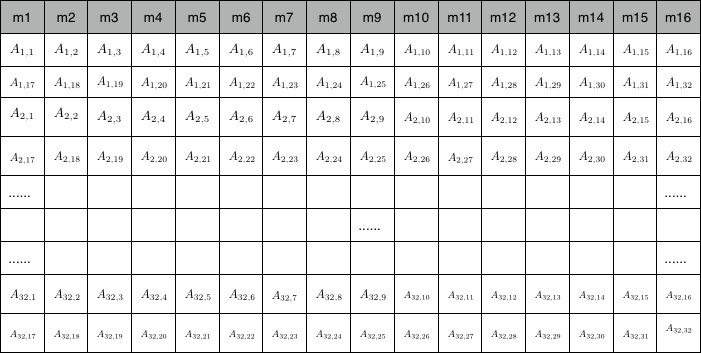
\includegraphics[scale=0.5]{row.png}
\end{center}
\end{figure}
(2) one column at a time \\
Actually, in this case it is similar with above one. In order to retrieve one column at time, all we need to do is store each element in one column into different memory modules, like store $A_{1,2}$ into $m_{1}$, $A_{2,2}$ into $m_{2}$ et al. \\
\begin{figure}[]
\begin{center}
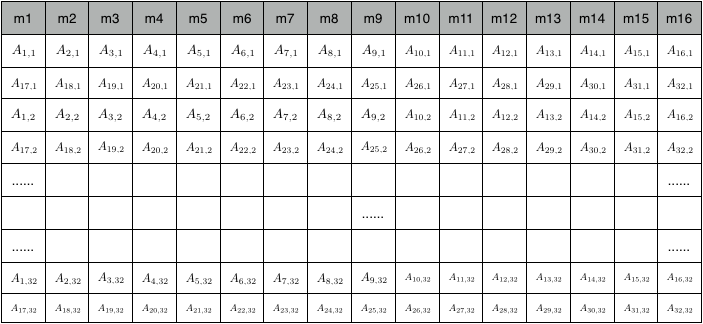
\includegraphics[scale=0.5]{column.png}
\end{center}
\end{figure}
(3) either a row or a column at a time \\
In this case, I just store the element like the following figure.
\begin{figure}[]
\begin{center}
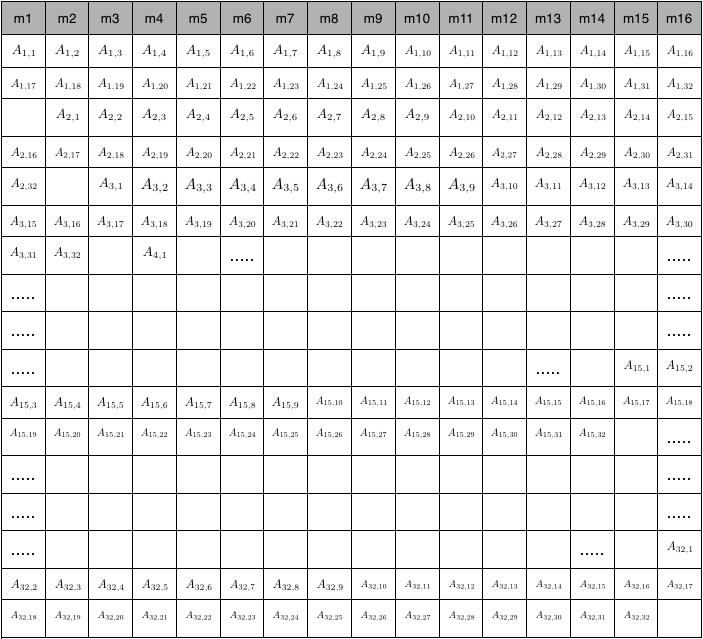
\includegraphics[scale=0.5]{row_column.png}
\end{center}
\end{figure}
Between each new row, there is a gap, so that we can retrieve either one row or one column simultaneously. The extra work here just involves the offset computation for each element.
\end{document}